% Diagram for the report (states). Build: see build.sh in this folder.
\documentclass[12pt]{standalone}
% Shared style of every diagram and chart in the report.
% Each agent keeps the same colour in every figure.
% The diagrams are drawn here, not in main.tex, so the report itself does not
% load TikZ: it includes the built PDFs and compiles within Overleaf's time limit.
\usepackage{amsmath,amssymb}
\usepackage{xcolor}
\usepackage{tikz}
\usetikzlibrary{positioning,arrows.meta,shapes.geometric,shapes.misc,fit,calc,backgrounds}
\usepackage{pgfplots}
\pgfplotsset{compat=1.18}

% Same text width as the report (A4, 30 mm + 20 mm margins), for the charts.
\setlength{\textwidth}{160mm}
\newcommand{\Rs}{Rs.\,}
\newcommand{\code}[1]{\texttt{\detokenize{#1}}}

\definecolor{ink}{HTML}{2B2B2B}
\definecolor{agAfill}{HTML}{E4F2E1}\definecolor{agAline}{HTML}{3E7D3A} % Agent 1 Document & Vendor
\definecolor{agBfill}{HTML}{FCEBD5}\definecolor{agBline}{HTML}{B8701D} % Agent 2 Approval & Inventory
\definecolor{agCfill}{HTML}{EEE4F4}\definecolor{agCline}{HTML}{6E4A8E} % Agent 3 Contract & Risk
\definecolor{agDfill}{HTML}{FBE4E4}\definecolor{agDline}{HTML}{A8474B} % Agent 4 Platform
\definecolor{infill}{HTML}{E8EDF6}\definecolor{inline}{HTML}{4F6188}    % infrastructure / data
\definecolor{exfill}{HTML}{F2F2F2}\definecolor{exline}{HTML}{6F6F6F}    % people and external systems
\definecolor{humfill}{HTML}{FFF6D6}\definecolor{humline}{HTML}{9A7B12}  % human decision points
\definecolor{chartA}{HTML}{9AA5B1}\definecolor{chartB}{HTML}{3F5E8C}    % chart: baseline / shipped

\tikzset{
  >={Stealth[length=2mm]},
  every picture/.style={font=\footnotesize, line width=0.6pt, draw=ink, text=ink},
  nohyph/.style={execute at begin node={\hyphenpenalty=10000\exhyphenpenalty=10000}},
  box/.style={nohyph, draw, rounded corners=2pt, align=center, inner sep=3pt, minimum height=8mm},
  agA/.style={box, fill=agAfill, draw=agAline},
  agB/.style={box, fill=agBfill, draw=agBline},
  agC/.style={box, fill=agCfill, draw=agCline},
  agD/.style={box, fill=agDfill, draw=agDline},
  infra/.style={box, fill=infill, draw=inline},
  ext/.style={box, fill=exfill, draw=exline},
  human/.style={box, fill=humfill, draw=humline},
  decision/.style={nohyph, diamond, aspect=2.2, draw=humline, fill=humfill, align=center, inner sep=1pt},
  flow/.style={->, draw=ink},
  dflow/.style={->, draw=ink, dashed},
  lbl/.style={font=\scriptsize\itshape, fill=white, inner sep=1pt},
  note/.style={font=\scriptsize\itshape, align=center},
}
\pgfplotsset{
  reportbars/.style={
    ybar, width=0.95\textwidth, height=6cm, ymin=0,
    enlarge x limits=0.18, bar width=11pt,
    ymajorgrids, grid style={draw=black!12},
    axis line style={draw=black!60}, tick style={draw=black!60},
    legend style={draw=none, font=\footnotesize, legend columns=-1, at={(0.5,1.03)}, anchor=south},
    tick label style={font=\footnotesize}, label style={font=\footnotesize},
    nodes near coords, every node near coord/.append style={font=\scriptsize},
    /tikz/every even column/.append style={column sep=0.6cm},
    legend image code/.code={\draw[#1, draw=none] (0cm,-0.1cm) rectangle (0.3cm,0.1cm);},
  },
}

\begin{document}
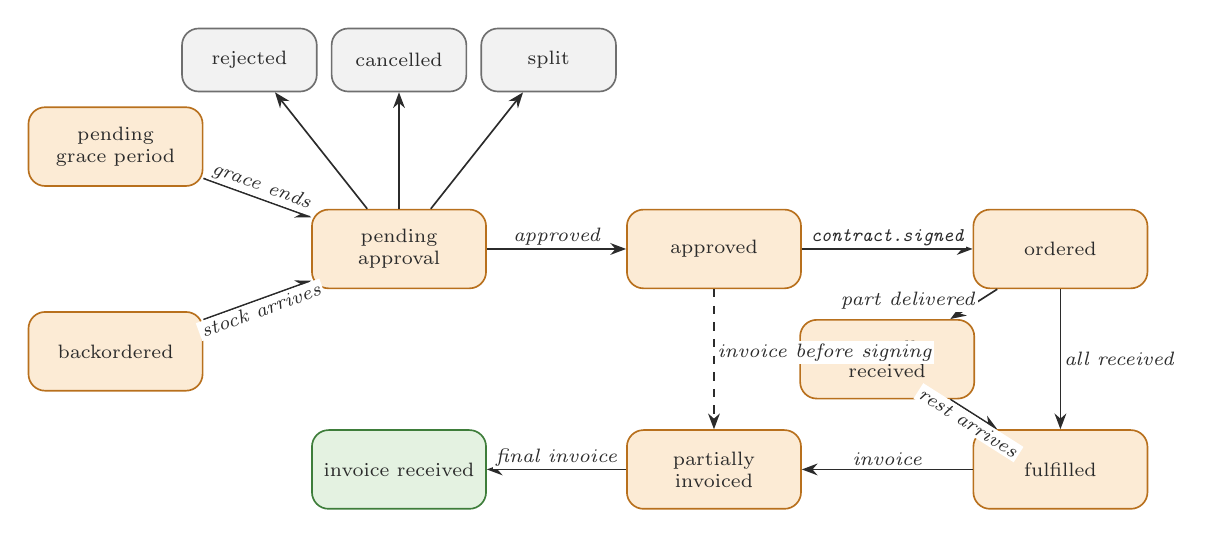
\begin{tikzpicture}
\tikzset{stt/.style={box, fill=agBfill, draw=agBline, rounded corners=6pt, text width=2.0cm, minimum height=10mm, font=\scriptsize}, term/.style={box, fill=exfill, draw=exline, rounded corners=6pt, text width=1.5cm, minimum height=8mm, font=\scriptsize}, tl/.style={lbl, font=\scriptsize\itshape}}
\node[stt] (gp) at (-7.0,1.9) {pending grace period};
\node[stt] (bo) at (-7.0,-0.7) {backordered};
\node[stt] (pa) at (-3.4,0.6) {pending approval};
\node[stt] (ap) at (0.6,0.6) {approved};
\node[stt] (or) at (5.0,0.6) {ordered};
\node[stt] (fu) at (5.0,-2.2) {fulfilled};
\node[stt] (prc) at (2.8,-0.8) {partially received};
\node[stt] (pi) at (0.6,-2.2) {partially invoiced};
\node[stt, fill=agAfill, draw=agAline] (ir) at (-3.4,-2.2) {invoice received};
\node[term] (rj) at (-5.3,3.0) {rejected};
\node[term] (cn) at (-3.4,3.0) {cancelled};
\node[term] (sp) at (-1.5,3.0) {split};
\draw[flow] (gp) -- node[tl, above, sloped] {grace ends} (pa);
\draw[flow] (bo) -- node[tl, below, sloped] {stock arrives} (pa);
\draw[flow] (pa) -- node[tl, above] {approved} (ap);
\draw[flow] (ap) -- node[tl, above] {\code{contract.signed}} (or);
\draw[flow] (or) -- node[tl, right] {all received} (fu);
\draw[flow] (or) -- node[tl, left, pos=0.4] {part delivered} (prc);
\draw[flow] (prc) -- node[tl, below, sloped] {rest arrives} (fu);
\draw[flow] (fu) -- node[tl, above] {invoice} (pi);
\draw[flow] (pi) -- node[tl, above] {final invoice} (ir);
\draw[flow] (pa) -- (rj); \draw[flow] (pa) -- (cn); \draw[flow] (pa) -- (sp);
\draw[dflow] (ap.south) -- node[tl, right, pos=0.45] {invoice before signing} (pi.north);
\end{tikzpicture}
\end{document}
